\documentclass{article}
\usepackage[utf8]{inputenc}
\usepackage{fullpage}
\usepackage{float}
\usepackage{graphicx}
\usepackage{gensymb}
\usepackage{amsmath}
\usepackage{amssymb}

\title{Chapter 9: Antenna Over Ground Planes}
\author{Rohit Singh}
\date{June 2022}

\begin{document}

\maketitle

\section{Pre-Lecture Notes}

\subsection{Antennas Over Ground Planes}

In many practical scenarios, an antenna is positioned above an \textbf{infinite half} space, meaning a medium (aside from air) which specific medium parameters such as $\sigma, e_r, \mu_r$. When we deal with ground planes, we are most often dealing with either:
\begin{itemize}
    \item Earth (high conductivity)
    \item Water (either salty or unsalty)
    \item Cement / Concrete
    \item Sand
    \item Mud
\end{itemize}

To study the behavior of antennas (input impedance and directivity/gain), we can make simplifying assumptions. If the conductivity of the medium is very high at the operating frequency of the antenna, we can model it as a \textbf{perfectly conducting surface} (that is, $\sigma \to \infty$). With this assumption, we can invoke image theory to yield results with good accuracy.

\subsection{Infinite Conductivity Ground Plane}

The specific \textbf{position} and \textbf{orientation} of the antenna is important in the sense that the equivalent problem is directly dependant on them.

We will consider two specific orientations, \textbf{vertical} and \textbf{horizontal}, from which form the basis that all orientations can be solved for using superposition.

\subsubsection{Case I: Vertical Position}

Invoking image theory, we can replace the antenna above a PEC ground with the two antennas shown here: 

\begin{figure}[H]
  \centering
     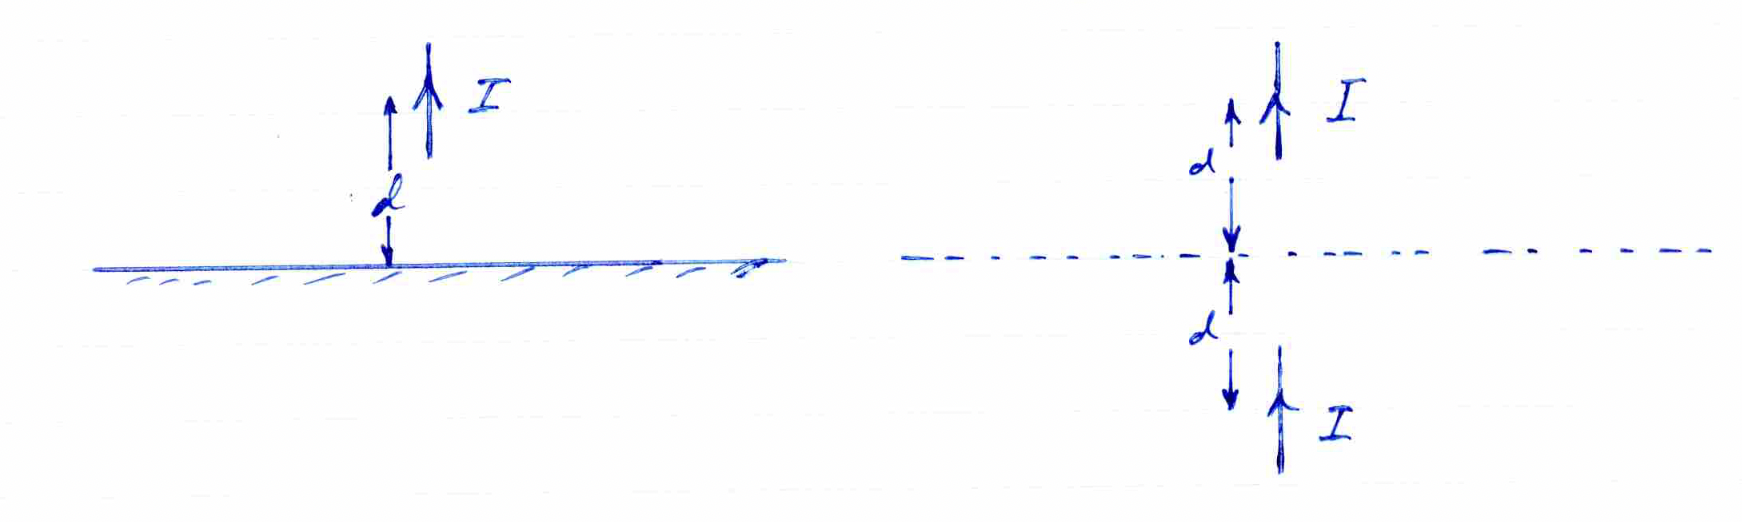
\includegraphics[scale=0.4]{Course Notes/images/9.1.png}
  \caption{Vertical Antenna over PEC (left) with its imaged counterpart (right)}
\end{figure}

Notice that the direction / phase of the image current is the same as on both halves of the reflection point (for vertical imaging, current direction is \textbf{in phase})

Now, let's assume that the antenna is a Herzian Dipole. We can construct the pattern of the equivalent system (the two antennas) by adding the electric fields of the two antennas.

\begin{figure}[H]
  \centering
     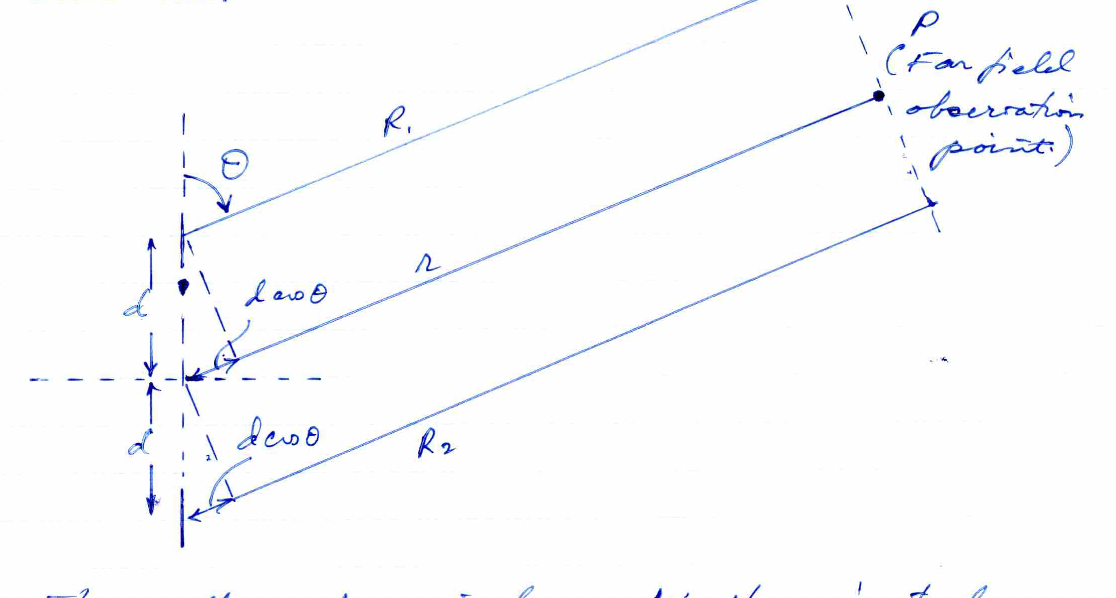
\includegraphics[scale=0.4]{Course Notes/images/9.2.png}
  \caption{Diagram reference to calculate electric fields of the two antennas}
\end{figure}

The pattern of a single vertically oriented Herzian Dipole is

\begin{center}
    $F_1(\theta) = A sin(\theta) \frac{e^{-j \beta r}}{r}$
\end{center}

By shifting the Herzian dipole above and below the center, the combined pattern becomes:

\begin{center}
    $F(\theta) = F_1(\theta) + F_2(\theta)$ \\ 
    \hspace{} \\
    $F(\theta) = A \sin(\theta) [\frac{e^{-j \beta R_1}}{R_1} + \frac{e^{j \beta R_2}}{R_2}]$ \\
    \hspace{} \\
    $F(\theta) = A \sin(\theta) [\frac{e^{-j \beta (r-d\cos(\theta))}}{R_1} + \frac{e^{j \beta (r + d \cos(\theta))}}{R_2}]$ \\
    \hspace{} \\
    Since: $R_1 = r - d\cos(\theta), R_2 = r + d\cos(\theta)$
\end{center}

We can make a slight approximation that $R_1 \approx R_2 \approx r$ \textbf{for the denominator only}. We only make this assumption for the denominator since the denominator terms that are dependant on radius only affect the magnitude of the field, and does so negligibly. The numerator terms affect the phase of the field and should therefore not be nullified.

\begin{center}
    $F(\theta) = A \sin(\theta) \frac{e^{-j\beta r}}{r} [e^{-j \beta (r-d\cos(\theta))} + e^{j \beta (r + d \cos(\theta))}]$ \\
    \hspace{} \\
    $F(\theta) = 2A \frac{e^{-j\beta r}}{r}[\sin(\theta) \cos(\beta d \cos(\theta))]$
\end{center}

Suppose we design our antenna such that $d = \frac{\lambda}{4}$, then when $\theta = 0$, we have $F(\theta) = 0$ due to the sin term, and when $\theta = 90 \degree \implies F(\theta) = 2F_1(\theta)$. This is intuitive, as we know that we should be perpindicular to the current if to witness the strongest E fields, not parallel.

\subsection{Case II: Horizontal Dipole}

Let us now consider a horizontal Herzian Dipole above a PEC.

\begin{figure}[H]
  \centering
     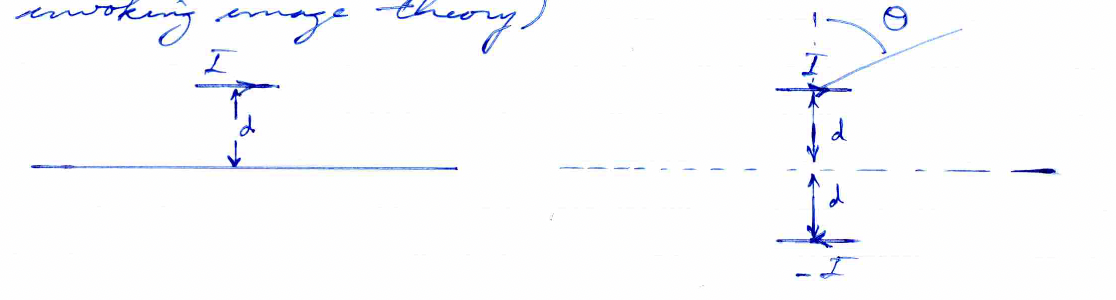
\includegraphics[scale=0.4]{Course Notes/images/9.3.png}
  \caption{Horizontal Antenna over PEC (left) with its imaged counterpart (right)}
\end{figure}

Using the same calculation procedure as before, the combined radiation pattern is found to be:

\begin{center}
    $F(\theta) \approx \cos(\theta) \sin(\beta d \cos(\theta))$
\end{center}

Note the similarities, only now our outer cos and sine terms are swapped. From this, when $\theta = 0 \implies F(\theta) = sin(\beta d)$ and $\theta = 90 \degree \implies F(\theta) = 0$. This means, if we are perpindicular to the vertical axis, there is no field! This is due to the opposing currents cancelling the induced E fields of one another.

\subsubsection{Case III: Non-PEC}

Assume the ground plane has finite conductivity, ($\sigma \ne 0$ and $\epsilon_r \ne 1$). In this scenario, we have to carefully pay attention to the plane over which we are observing the radiation.

Let's consider the vertical Herzian Diple. If the ground non-ideal, then we \textbf{cannot} replace the vertically-oriented current with itself and an image! However, suppose we are observing the field in the far field, then we can make a highly accurate approximation using what is referred to as \textbf{ray tracing}

\begin{figure}[H]
  \centering
     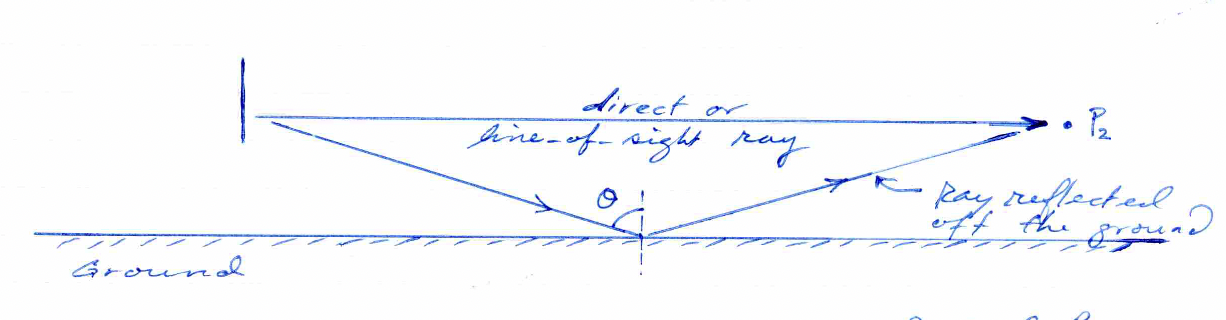
\includegraphics[scale=0.6]{Course Notes/images/9.4.png}
  \caption{Non-PEC rays}
\end{figure}

At any of our observation points, on the far field reaches these points. The far field reaching $P_2$ is represented by the direct (\textit{line-of-sight}) field and a field reflected off the ground.

Notice that the diagram above is deceptive in the sense that if $P_2$ is in the far field, then all the rays should be \textbf{parallel}. Suppose instead we neglect the horizon and consider the problem as drawn below:

\begin{figure}[H]
  \centering
     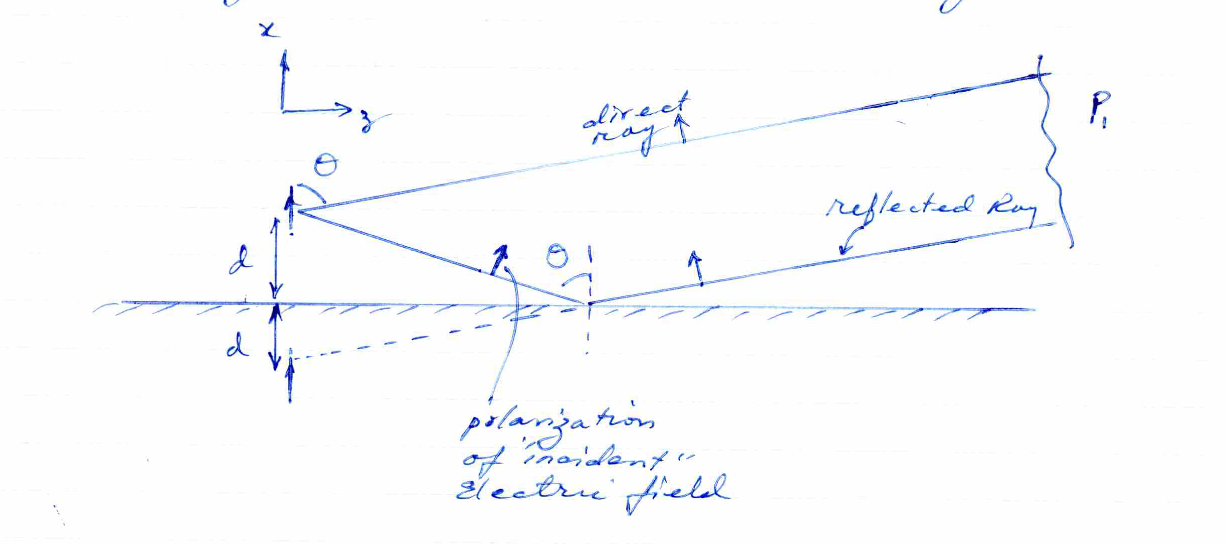
\includegraphics[scale=0.45]{Course Notes/images/9.5.png}
  \caption{Non-horizon formulation of Non-PEC problem}
\end{figure}

Using the analysis shown above, the far field will consist of two rays (or fields). 
\begin{enumerate}
    \item \textbf{Direct / LOS ray}
    \item \textbf{Reflected ray}:
    \begin{itemize}
        \item This ray has the same magnitude as the direct ray, except it is scaled by the reflection coefficient of a field polarized in the plane of observation (x-z plane in this case). 
        \tiem This particular field polarization is referred to as the \textit{H-Pol}, because the corresponding H-field is only in the y direction. 
    \end{itemize}
\end{enumerate}

We express the reflection coefficient by $\Gamma_v$. Now, we can consider this problem to be equivalent to one where the ground plane is replaced by an image with magnitude $I\Gamma_v$

\begin{center}
    $\Gamma_v = \frac{\epsilon_r' \cos(\theta) - \sqrt{\epsilon_r' -\sin^2(\theta)}}{\epsilon_r' \cos(\theta) + \sqrt{\epsilon_r' -\sin^2(\theta)}}$
    \\ \hspace{} \\
    Where: $\epsilon_r' = \frac{\epsilon'}{\epsilon_0} = \epsilon_r - j\frac{\sigma}{\omega\epsilon_0}$
\end{center}

For a horizontally oriented dipole, this same analysis as above applied, however we would have to introduce a $180 \degree$ phase shift in the magnitude of the equivalent current, due to the image theory rules.

Therefore, for a vertically oriented dipole, we have:

\begin{center}
    $F(\theta) \approx \sin(\theta)(e^{j\beta d \cos(\theta)} + \Gamma_v e^{-j \beta d \cos(\theta)})$
\end{center}

And for a horizontally oriented dipole, we have:

\begin{center}
    $F(\theta) \approx \cos(\theta)(e^{j\beta d \cos(\theta)} - \Gamma_v e^{-j \beta d \cos(\theta)})$
\end{center}

\subsection{Radiation Pattern in the x-y plane}

When placing a vertically-polarized anetnna above a ground plane, irrespective of the plane of radiation we are considering, the analysis above applied since the ray incident upon a ground plane is H-polarized.

However, for the case of the horizontally oriented dipole, the incident field has a different polarization which is E-polarization, since there is only one component of the E field and it's in the z-direction.

We can better understand this reflection phenomenon in the xy plane by considering the diagram below:

\begin{figure}[H]
  \centering
     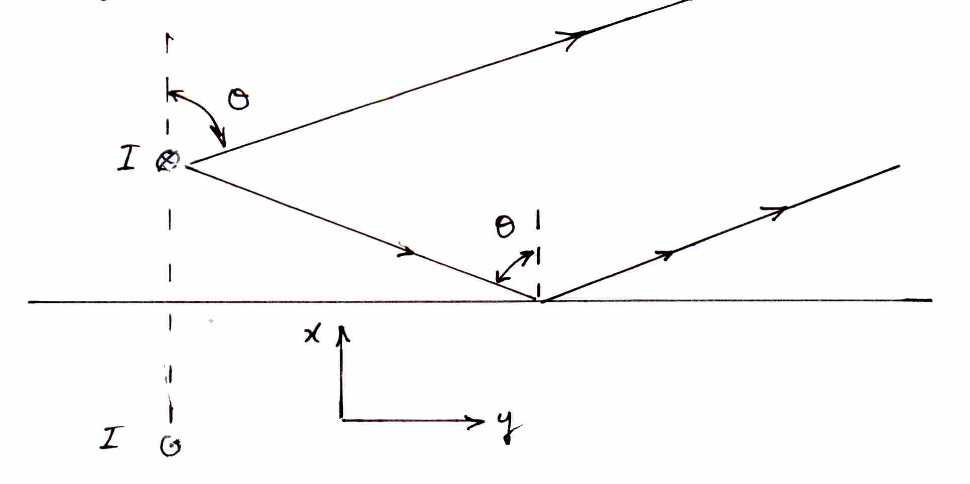
\includegraphics[scale=0.45]{Course Notes/images/9.6.png}
  \caption{Reflection Phenomenon Reference Diagram}
\end{figure}

In the xy plane, the only component of E is in the z-direction, which is perpendicular to the xy plane. This is referred to as E-pol.

\end{document}